\documentclass[12pt]{scrartcl}

%\usepackage[
%HomeHTMLFilename=index,     % Filename of the homepage.
%%HTMLFilename={node-},       % Filename prefix of other pages.
%%IndexLanguage=english,      % Language for xindy index, glossary.
%latexmk,                    % Use latexmk to compile.
%%   OSWindows,                  % Force Windows. (Usually automatic.)
%mathjax,                    % Use MathJax to display math.
%]{lwarp}


\usepackage{graphicx}
%\usepackage{subcaption}
\usepackage{float}
%\usepackage[nottoc,numbib]{tocbibind}
\usepackage{caption}
\usepackage[backend=bibtex]{biblatex}% Sort by citation order

\addbibresource{references.bib}


%\newcommand{\email}[1]{\texttt{\href{mailto:#1}{#1}}}

%\title{ENGR 446: Milestone Report I: Project Background}
%\author{David Li\footnote{Undergraduate student, Department of Electrical and Computer Engineering, University of Victoria, \email{lidavid@uvic.ca}}}

%\makeatletter
%\let\inserttitle\@title
%\let\insertauthor\@author
%\makeatother


%% Print Title Page
\makeatletter
% Create \printauthor command which will display contact info                     
\def\printauthor{%                  
	{\large \@author}}              
\makeatother
% Honestly, if footcite works that would be adequate for me
\author{%
	\textbf{Name: }  David Li \\
	\textbf{Student Number:} V00818631	\\
	\textbf{Year}  Fourth Year Student  \\
	\textit{Discipline:} Computer Engineering \\  \vspace{4pt}
	\textit{Email:} \href{mailto:lidavid@uvic.ca}{lidavid@uvic.ca}
}

%\bibliography{references.bib}

\usepackage[table]{xcolor}
\usepackage{tabularx}		% Tabulars with adjustable-width columns
\definecolor{lightgoldenrodyellow}{rgb}{1, 0.93, 0.55}
\definecolor{firebrick}{rgb}{0.7, 0.13, 0.13}
\definecolor{gray}{rgb}{0.5, 0.5, 0.5}
\definecolor{almostWhite}{rgb}{0.95, 0.95, 0.95}
\definecolor{purpleMix}{rgb}{0.35, 0.07, 0.57}
\newcommand*{\arraycolor}[1]{\protect\leavevmode\color{#1}}
\newcolumntype{A}{>{\columncolor{blue!50!white}}c}
%\newcolumntype{B}{>{\columncolor{lightgoldenrodyellow}}c}
\newcolumntype{B}{>{\columncolor{purpleMix!75}}c}
\newcolumntype{C}{>{\columncolor{firebrick!50}}c}
\newcolumntype{D}{>{\columncolor{lightgoldenrodyellow}}c}
\newcolumntype{E}{>{\columncolor{white!60!purple!20!green!20}}c} 

\newcommand{\foo}{\color{blue}\makebox[0pt]{\textbullet}\hskip-0.5pt\vrule width 1pt\hspace{\labelsep}}

\usepackage{kpfonts}	    % Fonts used in the title page

\newcommand{\onlineCite}{[Online] Available: }	% Used in BIBLIOGRAPHY

\usepackage{tikz}

\usepackage{booktabs}
\usepackage{hyperref}

\begin{document}

\makeatletter
% Create \printauthor command which will display contact info                     
\def\printauthor{%                  
	{\large \@author}}              
\makeatother
\author{%
	David Li \\
	V00818631	\\
	%Term 3B \\
	Computer Engineering \\  
	%\vspace{4pt}lidavid@uvic.ca 
}

%\maketitle

% Picture from https://pixabay.com/en/blockchain-block-chain-technology-3019120/

\begin{titlepage}
 \begin{tikzpicture}[remember picture, overlay]
  \node[opacity=0.05,inner sep=0pt] at (current page.center)
   {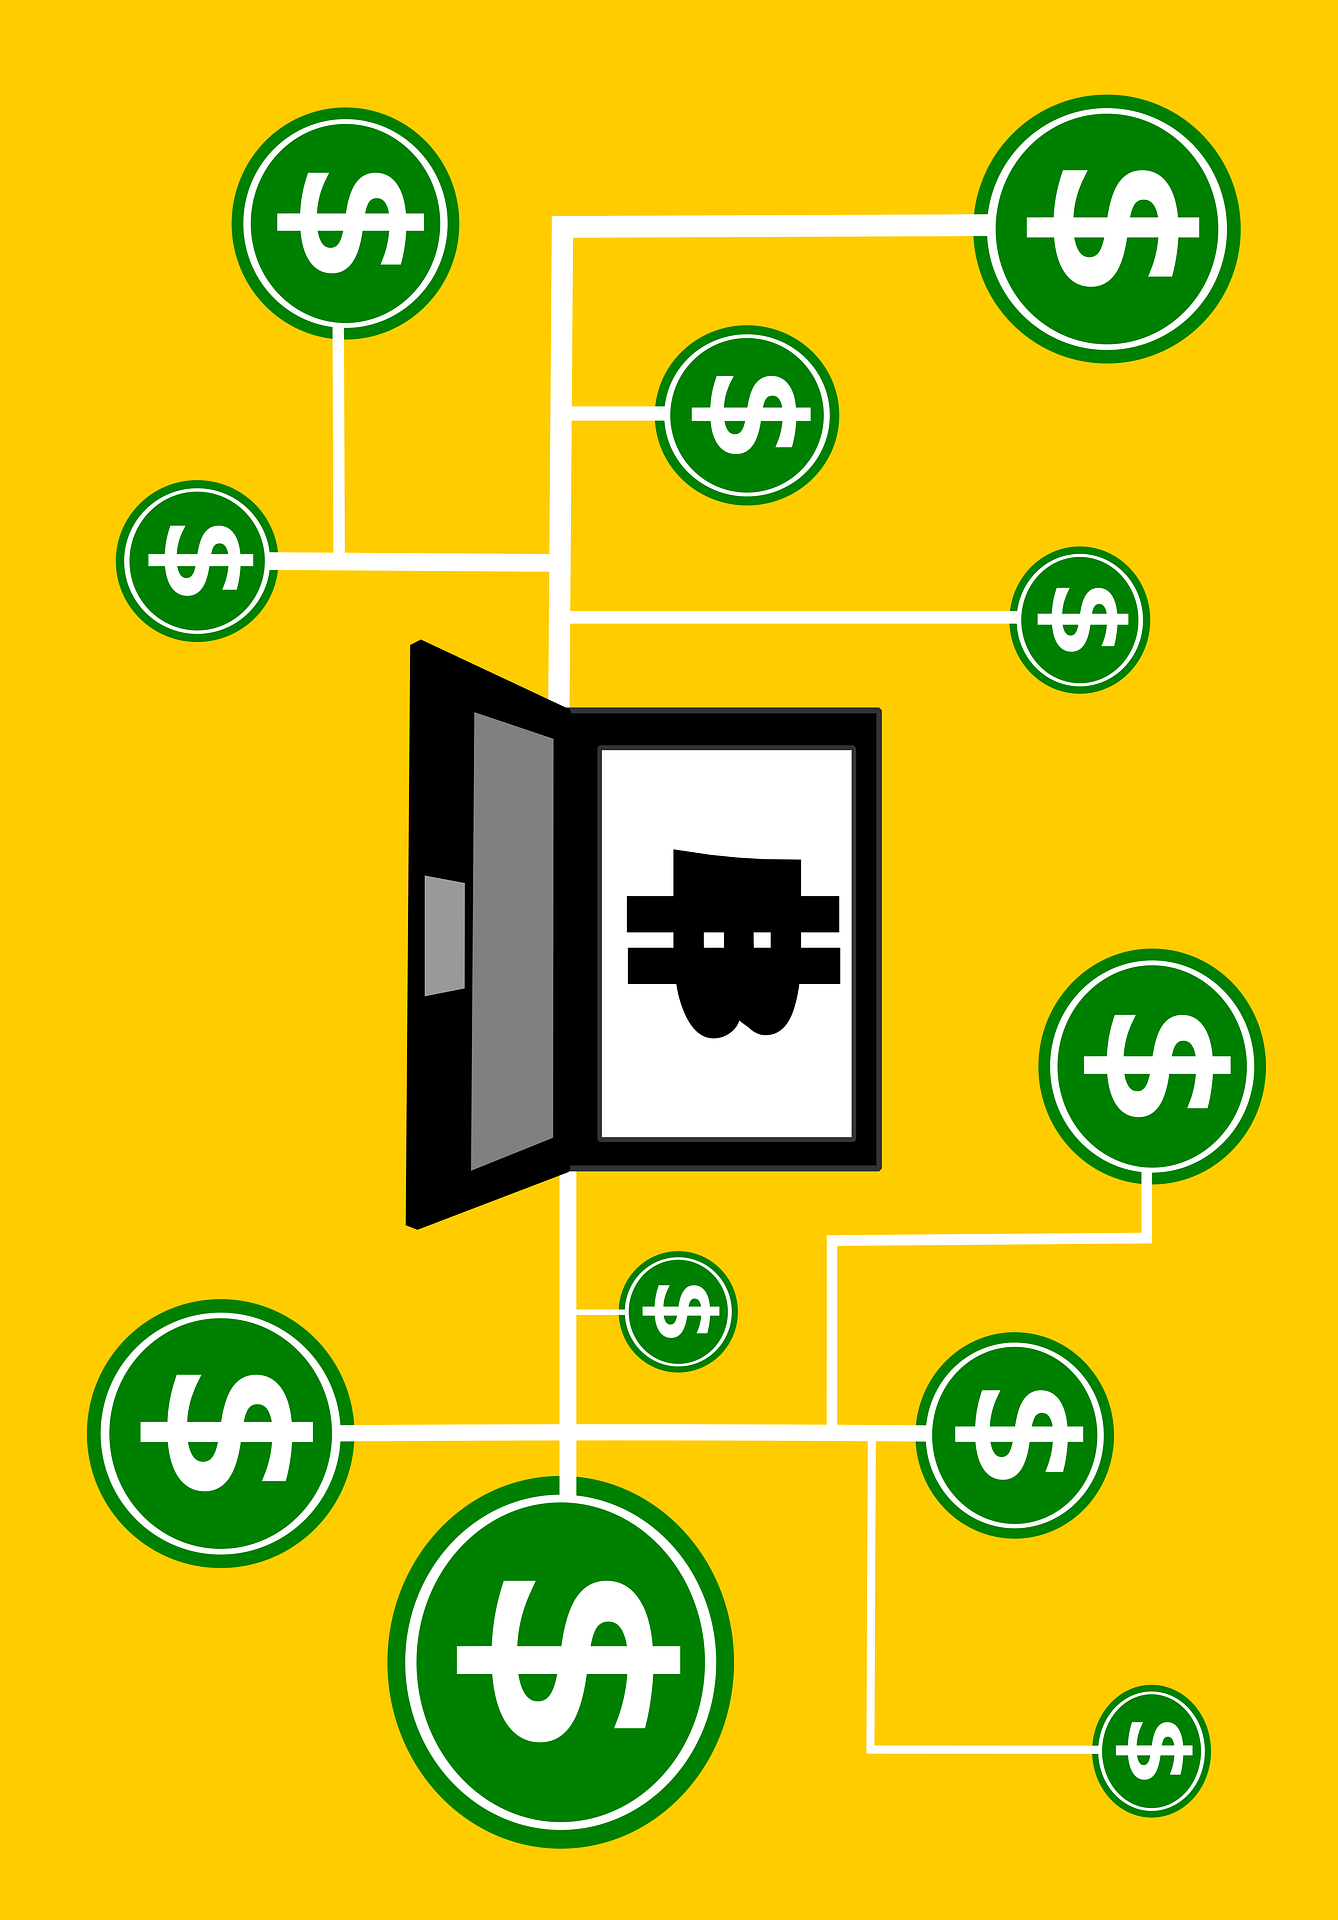
\includegraphics[width=\paperwidth,height=\paperheight]{bchainCOol.png}};
  \end{tikzpicture}
	\begin{center}
		{\vspace*{3pt} }
		{\Large University of Victoria \\ \vspace{4pt}}
		{\Large Faculty of Engineering \\ \vspace{4pt}}
		{\Large ENGR 446: Milestone Report I: Project Background \\ \vspace{4pt}}  
		\rule[13pt]{1\textwidth}{1pt} \\ \vspace{1pt}
		{\LARGE \textbf{{Simplification of Transactions by Leveraging Blockchain Technologies and Smart Contracts}} \\ \vspace{15 pt}}
		
		{\Large David Li \hfill Computer Engineering \hfill  V00818631 }
		%{\Large BC Ministry of Transportation and Infrastructure \\} 
		%					\vspace{4pt}} 
		%{\Large Information Management Branch}
		%	\vspace{4pt}}
		%{\Large Victoria, British Columbia, Canada \\ \vspace{60pt}}
		%\AddToShipoutPicture*{\BackgroundPic}
	%	\vspace{10pt}
		%\begin{minipage}

		%{\vspace{60pt} \\}
		%{\vspace{60pt}}
		{\vspace*{-20pt}}
		\begin{figure}[htb]
		\centering
		\makebox[0pt][c]{%
		\begin{minipage}{0.59\linewidth}
		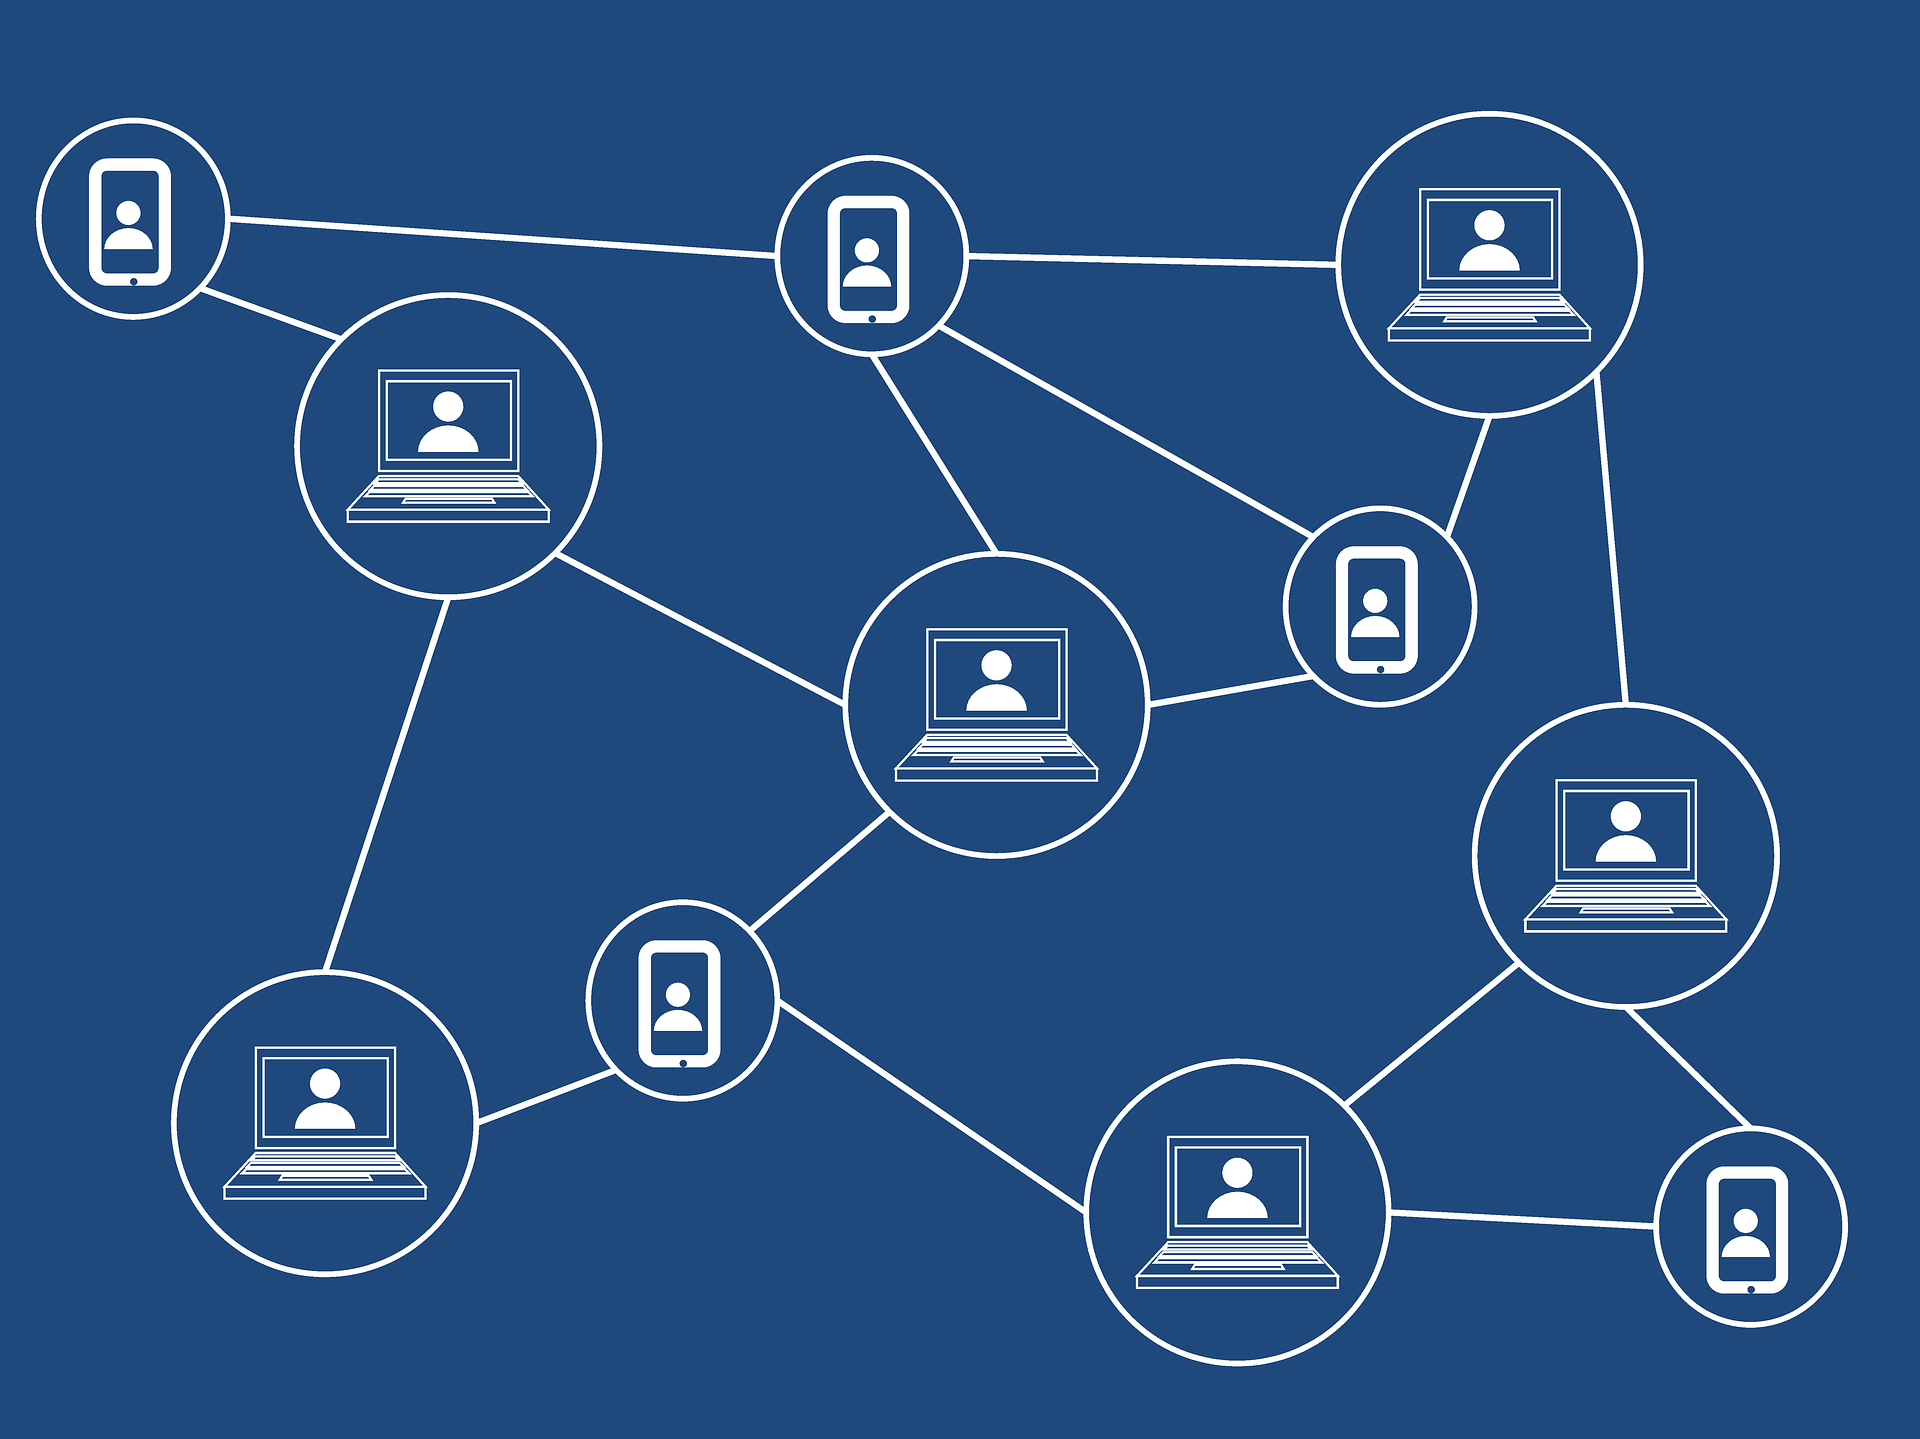
\includegraphics[width=1\linewidth,%
		  		keepaspectratio]{bchain.png}
		\end{minipage}
		\begin{minipage}{0.59\linewidth}
		
\includegraphics[width=1\linewidth,%
				  keepaspectratio]{bitcoinImageTrans.png}
		\end{minipage}%
		}%
		\end{figure}
%		\begin{minipage}{0.96\linewidth}
%			\begin{flushright}
%				\printauthor
%			\end{flushright}
%		\end{minipage}
%		\begin{minipage}{0.02\linewidth}
%			\rule[0pt]{1pt}{70pt} 
%		\end{minipage}

	%	\vspace{40pt}
		{\Large \today \\ \vspace{10pt}}
			{\Large In partial fulfillment of the academic requirements of this academic course}
	\end{center}%	\AddToShipoutPicture*{\fpict}
\end{titlepage}

\renewcommand{\contentsname}{Table of Contents}
\tableofcontents
\listoffigures
\listoftables

\newpage 
\section{Background}

In 2008 bitcoin white paper \cite{bitcoinWhitePaper:Online} described a way to solve the double spending problem without a centralized body using blockchain. Initially, used for cryptocurrencies, the applications of blockchain are numerous including revolutionizing transactions, video games \cite{loomNetwork:Online} and supply chains. Although, the value of bitcoin (BTC) has grown exponentially, high computational, energy consumption in mining and slow performance \cite{bitCoinProblems:Online}.  Released in July 30, 2015, Ethereum, an open-source platform based on blockchain technology, distinguishes itself from bitcoin through faster transactions, unlimited processing capability for smart contracts, and optimized to support Decentralized Applications \cite{ethereumWhitePaper:Online}.

%modify this for markdown file
\begin{table}[ht]
\centering
\renewcommand\arraystretch{1.4}\arrayrulecolor{blue}
%\captionsetup{singlelinecheck=false, labelfont=sc, labelsep=quad}
\caption{Timeline of Cryptocurrency}%\vskip -1.5ex
% lwarp table, and print edition (uncomment stuff below for good copy)
%\begin{tabular}{l l }%
% Good copy for print edition
\begin{tabular}{@{\,}r <{\hskip 2pt} !{\foo} >{\raggedright\arraybackslash}p{5cm}}
\toprule
%\hrule
%\addlinespace[1.5ex]
2008 & Bitcoin White Paper \\
2009 & Bitcoin Genesis Block\\
2013 & 1 BTC = \$ 31 USD\\
2013 & Ethereum White Paper \\
2015 & Ethereum Genesis Block\\
2015 & HyperLedger starts \\
2017 & Over 1000 different cryptocurrencies \\
2018 & AWS Blockchain Templates \\
\end{tabular}
\end{table}


Blockchain technology is revolutionizing the internet by establishing trust in shared data. \cite{ethereumWhitePaper:Online}.
	Additionally, transactions recorded on the blockchain are practically impossible to remove or change. 
	A decentralized application, or DApp are deployed on peer to peer networks such as Ethereum or on the cloud. Traditional legal contracts are written to represent the contracting parties. In a smart contract, self-executing source code is used to automatic transactions that are publicly available on the blockchain \cite{ethereumWhitePaper:Online}.

\begin{figure}[ht]
		\centering
		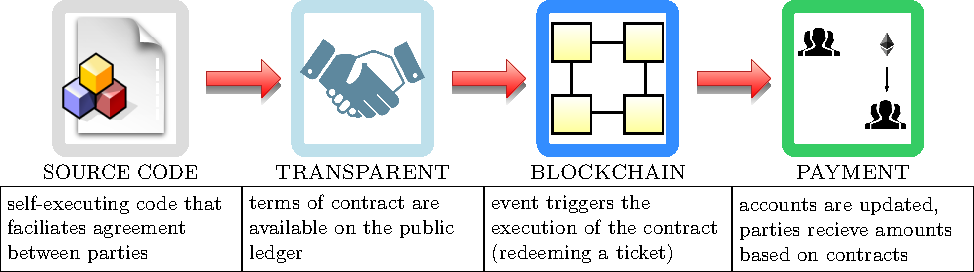
\includegraphics[width=1\linewidth]{smartContractsExp.pdf}
		\caption{Illustrating how a smart contract works}
		\label{fig:smartContracts}
\end{figure}

\newpage 

\section{Objective}
The prominence of cryptocurrency and decentralized applications suggests usage of smart contracts will experience explosive growth.

\subsection{Problem}

Currently commonplace transactions require days to process and for parties verify correctness. For example to purchase houses, a plethora of steps are required, one must interactive with lawyers, real-estate agents, home inspector, buy insurance and shop for a mortgage. 

\subsection{Purpose}
Leveraging existing blockchain technologies can automatic the majority of steps and cut out the middlemen, resulting in buyers conversing directing with sellers.
% Although smart contracts have immense potential to simplify transactions, issues such as limiting access to information, latency when updating (takes 10 minutes to write info to bitcoin blockchain), and immutability of translations (cannot undo transfer of assets) must be addressed.
% See https://www.cs.auckland.ac.nz/research/groups/ssg/homepages/yu-cheng/ytu001_PhDThesis.pdf
% https://researchspace.auckland.ac.nz/handle/2292/22092
\subsection{Aims}
The aims of this project are to develop a decentralized blockchain system that:
\begin{enumerate}
\item Reduce cost of transactions by at least 50\% from removing middlemen.
\item Improve transparency in software systems through augmented accessibility and understandability.
\item Has increased reliability and more secure than traditional systems.
%1. Uses 15% less material to decrease cost and weight.
%2. Has improved efficiency by reducing the air gap by 10%.
%3. Has no reduction in its reliability or increase in its maintenance requirements. 
\end{enumerate}
\subsection{Limitations}

The regulatory uncertainty and impact of future regulations on blockchain technologies such as smart contracts will not be investigated. In addition, criminal usage of cryptocurrencies to avoid taxation and legal repercussions are beyond the scope of this report. 
%The performance of the linear generator in extreme storm events will not be investigated as this
%cannot be accurately modeled using Airy linear wave theory. This project will be based on
%numerical simulations; no physical model will be tested to validate the results.

\newpage  
\section{Potential Solutions}

\begin{itemize}
	\item[---] \textbf{Public blockchains} are large distributed networks that are run through a native token such as bitcoin or ether. Anyone can participate and the community maintains its open-source code. The two largest public blockchains are Ethereum and Bitcoin. They are open for anyone to participate at any level and have open-source code that their community maintains.
	% rewrite and add section about composer
	\item[---] \textbf{Permissioned blockchains} define role based access control for individuals in the network and uses native tokens.  HyperLedger Composer, an open-source framework for permissioned blockchains, is used for smart contracts and for blockchain application development \cite{hyperledgerComposer:Online}. One use case is an accounting system that calculates payment, while hiding that information from unrelated organizations.  \hfill \break % Their core code may or may not be open source.
	\begin{figure}[ht]
	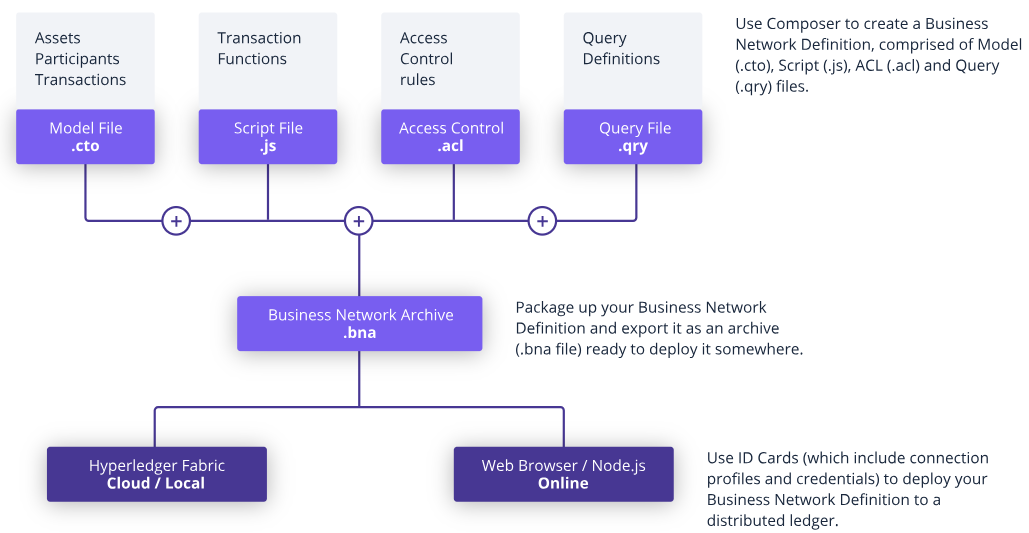
\includegraphics[width=1\linewidth]{composer-arch.png}
	\caption{Architecture of Hyperledger composer}
	\end{figure}
	\item[---] \textbf{Private blockchains}  membership is tightly controlled and lacks a native token. Useful for consortiums with trusted associates and exchanging confidential information, however, less powerful because it is supported by limited private resources. Large organizations such as governments will likely use these extensively.
\end{itemize}

\newpage 
\section{Initial Assessment}
% Discuss how it is significantly more accessible for money to issue their own currencies, ICOs

% Explain how much it costs to how a bunch, like 5%, getting an automatic system will be cheaper as wages will not be paid, cover cost of gas
% "Gas" is the name for a special unit used in Ethereum. It measures how much "work" an action or set of actions takes to perform: for example, to calculate one Keccak256 cryptographic hash it will take 30 gas each time a hash is calculated, plus a cost of 6 more gas for every 256 bits of data being hashed. Every operation that can be performed by a transaction or contract on the Ethereum platform costs a certain number of gas, with operations that require more computational resources costing more gas than operations that require few computational resources.

% https://ethereum.stackexchange.com/questions/3/what-is-meant-by-the-term-gas

Determining which platform is best for smart contracts should be done using a weighted decision matrix, based on the particular application. For internal processes such as supply chains, a private blockchain makes sense (data cannot be changed) and cryptographic auditing with known identities (public keys). For a trustless system that verifies every transaction, using a public blockchain is essential. In comparison, role-based access control is feasible by using a permissioned blockchain. \hfill \break
%\hfill \break 

Despite the slow speed of the public blockchain, innovations such as side chains enable quick transactions and are used in decentralized game development \cite{loomNetwork:Online}. A permissioned blockchain allows role based access control which is essential in business applications. One example is to prevent unrelated parties from viewing other's data. 	Furthermore, smart contracts allow buyers and sellers exchange money, property, shares, or anything of value in a transparent, conflict-free way while avoiding the services of a middleman. This allows validation of complex transactions swiftly while maintaining transparency.
%modify this for markdown file

\begin{table}[H]
\centering
\caption{Sample Decision Matrix for designing a blockchain system}
\arrayrulecolor{white}
\arrayrulewidth=1pt
\renewcommand{\arraystretch}{1.5}
\rowcolors[\hline]{3}{.!50!white}{}
\begin{tabular}{D E A B C }
\multicolumn{1}{l}{}      & \multicolumn{1}{c}{Existing Systems}    & \multicolumn{3}{c}{BlockChain Systems}                                                                                    \\
\multicolumn{1}{c}{Criteria}                 & \multicolumn{1}{c}{Centralized} & \multicolumn{1}{c}{Public} & \multicolumn{1}{c}{Permissioned} & \multicolumn{1}{c}{Private} \\
speed and latency         &    5                                     &      7                                 &         7                                    &                  6                     \\
scalability         &        5                                &     9  8                                &          7                                &                         4               \\
security and immutablity  &     3                                    &                        7               &    8.5                                         &                   9                     \\
storage capacity          &        4                                 &            9                           &                         9                    &         6                               \\
transparency              &   3                                      &                         9              &    7                                            &               5                         \\
\multicolumn{1}{c}{Total} &    21                                     &               41.6                        &    38.5                                         &          30                             
\end{tabular}
\end{table}

 A decentralized system (peer to peer) has many advantages over a conventional centralized network including no single points of failure, cheaper distribution (servers are expensive), faster upload speeds and improved security. In addition, irreversible and immutable transactions are both an advantage and disadvantage. For example, an amateur coder killed the contract that allowed users to transfer Ether for the Parity Ethereum Wallet, rendering 150 to 300 million dollars completely useless \cite{funnyJoke:Online}.
Overall, the public blockchain with access to substantial collective resources is most viable in terms of scalability and transparency, however, institutes may prefer implementing permissioned or private blockchains internally for extended security and privacy. 


\newpage 
% Add survey of functionality, what industries could be impacted A survey of potential users. 
\printbibliography

\end{document}